\chapter{Session attack countermeasures}

In this chapter, different countermeasures to the session hijacking and session fixation attacks are discussed, together with a detailed analysis of their shortcomings. We first describe some general security measures that a web developer can take to secure his web application. Next, we inspect different web frameworks to see how well they apply these principles. Afterwards, we give an overview of standalone countermeasures, both at the server side and at the client side, that were developed over the years. We close with a brief description of some solutions to cross-site scripting attacks, because of their importance in session attacks. We do not consider solutions to cross site request forgery here, since these would lead us too far.

\section{General security measures}\label{general-security}

Different security measures may be taken by web application and web framework developers to secure their web applications. In this section, we discuss to what extent these measures provide security against session hijacking and session fixation attacks.

\subsection{Renewing the session identifier}\label{renewing}

The practice of renewing the session identifier (see section \ref{renewing-sid}) can provide excellent protection against \gls{login session fixation} attacks. Indeed, if the web application renews the session identifier every time the authentication status of a user changes, the SID which was enforced by the attacker won't be valid anymore once the victim has logged in. As an example, this can be accomplished in PHP by using the following code snippet \cite{PHPregenerate,Johns2011}:

\begin{lstlisting}[language=PHP]
if ($authentication_successful) {
    $_session["authenticated"] = true;
    session_regenerate_id();
}
\end{lstlisting}

To make sure that the session identifier is changed on every authentication change, it can be made to contain specific user information (like the username). In this case, when the authentication state changes, the session identifier has to change, too. If this is used in combination with a server \gls{mac} (as described by Fu et al. \cite{Fu2001}), an attacker is not able to include another username in the value himself.

Renewing the session identifier regularly is also benefical for preventing session hijacking attacks. As was discussed in section \ref{lifetime}, the shorter the lifetime of a session identifier, the more difficult it will be to capture, and the less useful it will be if it has been captured \cite{Fu2001}.

Keeping in mind the previous discussion, one might assume that it is best to renew a session identifier as often as possible. Consider, however, the case where the session identifier is renewed on each request. In this case, every request would result in a new session cookie being set at the user's browser, with the old session cookie being invalidated. When issuing concurrent requests (for example, when loading the images on a web page), the web application would only acknowledge the first request that arrived at the server. The second request would contain the (by then) invalidated session identifier, causing it to be rejected. Because of this, the browser would be allowed to issue only one request at the same time. Similarly, this would pose a problem when browser plugins communicate with the server, as well as with asynchronous requests. Another drawback of this approach is that web applications making use of multiple servers would have to synchronize their users' SID on every request \cite{Dacosta2011}. Otherwise, a user would have to re-authenticate every time a page is served by a different server. A last problem with this approach is that the server must issue an extra write to the database on every request, in order to update the SID.

\subsection{Using HttpOnly cookies}\label{httponly}

When setting a cookie in the user's browser, a web server can use the cookie's \texttt{HttpOnly} flag to indicate that the browser should only allow access to this cookie via \gls{http}. As a consequence, script code will not be able to access or edit the value for such cookie, and session hijacking via \gls{xss} attacks can be prevented \cite{HttpOnly}.

Session fixation, on the other hand, is \emph{not} solved by using \texttt{HttpOnly} cookies. Indeed, when the attacker sets the cookie before the web server does, \emph{he} is the one who can decide whether the \texttt{HttpOnly} flag is set. Thus, the web developer would have to make sure that a cookie is always set before an attacker can set it.

Moreover, even if the web server is able to set the session cookie before the attacker does, the attacker is still able to perform a successful session fixation attack via XSS. As Singh et al. have shown, it is sometimes still possible for an attacker to read or manipulate a HttpOnly cookie via JavaScript after it has been set \cite{Singh2010}. Fortunately, our experiments show that the issue of Firefox allowing cookie writes to HttpOnly cookies has since been solved.

Nevertheless, we discovered yet another technique which allows an attacker to circumvent the \texttt{HttpOnly} browser policy. As we described in section \ref{subdomain-setting}, the attacker is often still able to set a cookie with the same name as the session cookie for the parent domain. This causes the browser to send both the parent domain cookie and the subdomain cookie when a page on the subdomain is accessed. Since the \texttt{domain} attribute isn't attached to cookies in the request, the server has no way of distinguishing between the injected and the legitimate cookie. As such, we must conclude that, while marking a cookie as \texttt{HttpOnly} does prevent an attacker from accessing the cookie via JavaScript (thus mitigating the session hijacking attack via XSS for these cookies), it does not prevent him from using XSS to inject a chosen value for this cookie into the victim's browser.

\subsection{Secure connections}\label{ssl}

Secure (\gls{ssl}) connections \cite{Stallings2011} can be used to make sure that a session identifier can not be intercepted by a passive \gls{mitm} attacker. In this case, as already noted in \ref{secure-flag}, care must be taken that cookies can never be sent over an unsecure connection. This can be done by setting the \texttt{secure} flag for cookies that will be used only over a \gls{ssl} connection.

Recently, some work has been done to make deployment of HTTPS more widespread \cite{Hodges2010,Jackson2008}. Unfortunately, there are still some drawbacks to using HTTPS for every page \cite{Adida2008}. At the server side, HTTPS is very costly: every connection needs computationally intensive SSL operations to be performed. At the client side, browser caching works differently under SSL, and websites have to be completely transmitted before they can be rendered (because the validity is checked for the entire page).

\subsubsection{Checking other request headers}

Similar to the \texttt{Cookie} header we discussed in section \ref{cookie-header}, a \gls{http} request can contain many other headers \cite{rfc2616}. Some of these headers provide information that can be used to identify a user. For example, the \texttt{User-Agent} header contains information about a user's browser and operating system, while the \texttt{Accept-Language} header lists the languages the user is willing to receive.

A web server can gain some extra certainty about whether it is interacting with the user corresponding to the session ID in the request by comparing some of the header values to those in the last request with the same session ID. Indeed, because an attacker is probably using a configuration which is different from the victim's, the attacker's requests will have different header values. Thus, when certain header values differ between requests, it is possible that a session hijacking or session fixation attack occurred.

The question is then: which headers could be considered to give enough user-specific information, without changing over time? The \texttt{User-Agent} header is obviously the best candidate. Unfortunately, web proxies are known to modify this header \cite{ShiflettHijacking}. Another header which could be considered is the \texttt{Accept} header, which lists the types of content the user's browser will accept. The problem with this header is that in Internet Explorer, its value can change over time \cite{ShiflettHijacking}. The \texttt{Accept-Language} header could be considered. However, different browsers might have the same default value (\texttt{en-US}) for this header. The same goes for the \texttt{Connection} and \texttt{Cache-Control} headers. Other headers are too susceptible to change, and shouldn't be used.

Another problem with using HTTP headers for this purpose is that they are easily guessed by an attacker. Indeed, for most headers, only few options are possible, with even less options being very probable. Furthermore, even in the case that an attacker would not be able to guess the header values, he only needs to read a single request (to whatever server) from the victim to know what header values to use. He can get a request from the victim by intercepting it, or by tricking the victim into visiting his own website.

Thus, while checking the headers might raise the barrier for attackers, it is by no means a complete solution against any of the described session attacks.

\subsection{Checking the IP address}

Similar to request headers, the \gls{ip} address can be used by the web server to ensure it is interacting with the same user as before. Unfortunately, this approach also suffers from some problems. Firstly, IP addresses can be captured in much the same way as HTTP headers. An attacker can then easily change the source IP address for his own packets to impersonate the victim. Secondly, when both the victim and the attacker are behind the same \gls{nat} proxy (as is often the case in session hijacking attacks over a wireless network), they are using the same IP address \cite{Johns2011}. In this case, the server can not distinguish the attacker and the victim based on IP address. Lastly, requiring that the IP address stays the same over time can also cause some problems to the legitimate user: with users changing the location of their notebook or cell phone, the IP addresses of these devices will change when roaming, causing them to be denied access to a web application that checks their IP address. Moreover, some networks only issue dynamic IP addresses to their users. Because of these reasons, it can not be assumed that a user is uniquely tied to a single IP address.

As was the case for checking other request headers, checking the IP address can not be considered a complete solution to any session attack.

\subsection{Cookies vs. URL rewriting and form elements}\label{url-vs-cookies}

As we described in section \ref{session-management}, there are three major methods for doing session management: via \glspl{cookie}, via \gls{url} rewriting and via form elements. We compare the advantages and disadvantages of these methods here.

A first major disadvantage of URL rewriting was already discussed in section \ref{leaking-via-user}: the session identifier can leak when a link is shared with someone else (for example, via e-mail or a social networking site) \cite{Johnston2004}. A leak can also occur when the \texttt{referer} HTTP header is included in a request to another website: since the URL in the referer header contains the user's session identifier, this identifier is visible to the other website \cite{Fu2001}.

A disadvantage which is shared by both the `URL rewriting' and `form elements' methods is that the injection of a session identifier (with the objective of executing a session fixation attack) requires little effort from an attacker. Indeed, as we saw in section \ref{get-or-post}, such an injection attack is reasonably straightforward.

There is, however, also an advantage of choosing URL rewriting or form elements over cookies, in particular when looking at the cross site request forgery attack. Recall that, to execute a \gls{csrf} attack, an attacker tricks the victim's browser into issuing a request. For this, he  has to create a URL or a form containing the right GET/POST parameters for the attack. However, if the SID is one of the parameters that must be included in the request, the attacker does not know all required parameters, and is therefore not able to create a complete request \cite{Johnston2004}.

It is clear that choosing which method to use for managing sessions requires careful weighing of the advantages and disadvantages of each method. It could be argued that cookies provide more security since they make leaking of session identifiers less likely. Indeed, it is often recommended to use cookies instead of URL rewriting for session management \cite{Zhong2006,Vamosi2006}. An even better option is to use a combination of cookies and POST or GET parameters. As we will see in section \ref{xss-countermeasures}, this is what many CSRF countermeasures try to do \cite{Jovanovic2006,Johns2006}. In addition, some (mobile) web browsers don't support cookies, requiring the use of POST or GET parameters when session management is needed.

\subsection{Using an alternative to web sessions}

There are also other -- in some cases more secure -- methods for a web server to know which user it is interacting with. We describe three alternatives to web sessions here.

\subsubsection{Logging in for every request}
Arguably the most secure way to determine whether a user is who he claims to be, is to make him enter his credentials for every request. It is obvious that this is very cumbersome for the user, who has to log in every time he requests a new web page. It is, however, good practice to require the user to log in for certain actions \cite{Webers2008}. Indeed, consider the case where an attacker was able to take over a victim's temporary session. If no login is required to change the user's password, the attacker can completely take over the victim's account by changing the password to a value only he knows. Similarly, if the attacker is able to change the victim's e-mailaddress without having to enter the password, he can use the website's password recovery feature to have a password for the user's account sent to his own inbox.

\subsubsection{HTTP-Auth}
In HTTP Authentication \cite{rfc2617}, a separate HTTP header (called \texttt{Authorization}) is used to transfer the user's credentials on every request. These credentials are often cached by the browser to relieve the user from having to enter them on every request. A disadvantage of this approach is that the username and password are sent encoded (with the Base64 algorithm) but not encrypted, causing them to be available to a passive \gls{mitm} if no secured connection is used. Another disadvantage is that, since HTTP Authentication is completely handled by the HTTP stack, it is a much less flexible approach than web sessions. For example, there is no easy way for the user to log out, and the server-side HTTP stack needs full access to the user database \cite{Adida2008}.

\subsubsection{HTTP-Digest}
HTTP-Digest is a variant of HTTP-Auth that uses encryption instead of just Base64 encoding \cite{rfc2617}.This has the advantage that the user's credentials can not be intercepted by a passive MitM attacker. Unfortunately, this method is vulnerable to \emph{active} MitM attacks. It also suffers from the same inflexibility that is associated with HTTP-Auth.

\subsubsection{SSL client certificates}\label{certificates}
When secure sessions (see section \ref{ssl}) are used, mutual authentication can be achieved when both server and client possess a SSL certificate \cite{Park2000}. The problem with this approach is that many clients don't have certificates, and that certificate management is still too difficult for most regular users \cite{Whitten1999}. Moreover, a user needs to have its certificate installed on every device he wants to use to access the web application, which is not practical in the current world where people use smartphones and public computers to access web applications.

\section{Session security in web application frameworks}\label{frameworks}

Often, web applications are built on top of a web application framework. A \gls{web application framework} provides a web developer with the core functionality of a web application \cite{Schwartz2010}. This core functionality typically consists of elements like user session management, data persistence, and templating systems used to dynamically render web pages. It is upon the foundations provided by these frameworks that many dynamic web applications are built.

In this section, we describe the measures that are taken in some widely used frameworks to ensure security against session hijacking and session fixation attacks. We consider only the renewing of the SID, the use of secure connections, and the use of cookies or GET and POST parameters, because these are the security measures that are most eligible to be included in a web application framework. The list of frameworks is by no means complete \cite{FrameworksComparison}, but gives a good overview of how popular frameworks handle session attacks.

\subsection{Tomcat}

Apache Tomcat\footnote{More information about Tomcat is available on its website: \url{http://tomcat.apache.org/}.} is a much-used software implementation of the Java Servlet and JavaServer Pages technologies. It powers the websites of a.o. WalMart, Wolfram Research and CiteSeerX \cite{TomcatPoweredBy}.

Renewing of the session identifier on authentication is automatically done since Tomcat 6.0 \cite{TomcatAuthentication6}. In previous versions (since 5.5), it is possible to enable this behavior by setting the \texttt{changeSessionIdOnAuthentication} configuration attribute in Tomcat's Authenticator Valve \cite{TomcatAuthentication5}.

Tomcat uses cookies for session management, but also accepts SIDs that are included in the URL. URL rewriting is also used by default when the client's browser does not support cookies. It is possible for a web developer to disable this behavior, and to obligate Tomcat to only accept SIDs in cookies. This is, however, rather cumbersome, because it requires the implementation of a filter that intercepts requests and disables the session IDs from their URLs \cite{Condit2006}.

Secure connections can be managed managed by either the JSSE or the APR \gls{ssl} implementation. To enable Tomcat to use secure connections, the web developer must set the \texttt{protocol} attribute of the Connector configuration entry to use one of these two implementations \cite{TomcatSSL}. A cookie can be set with the \texttt{secure} flag by using the \texttt{setSecure()} method of the \texttt{Cookie} class \cite{TomcatCookie}. Session cookies that are set using a HTTPS connection automatically have the \texttt{secure} flag enabled \cite{Funk2004}.

\subsection{Alfresco}

Alfresco\footnote{More information about Alfresco is available on its website: \url{http://www.alfresco.com/}.} is a complete content management system that runs on a J2EE application server like Tomcat \cite{TomcatPoweredBy}. It is used by companies like France AirForce, Cisco, Fox and KLM \cite{AlfrescoPoweredBy}.

Alfresco neglects to renew a user's session identifier when he logs in. We tested the behavior using Alfresco's demo server\footnote{An account for the demo server can be obtained from \url{http://www.alfresco.com/try/}.} and found that a session fixation attack is, indeed, possible. Further investigation showed that a bug which addresses this issue was already reported \cite{AlfrescoSessionFixation}. Unfortunately, the bug already dates from October 2008 and has not been solved since. Requesting more information about session management in Alfresco on their \gls{irc} channel or in the Alfresco forums proved fruitless.

If Alfresco is deployed on top of Tomcat, session management and secure connections work in much the same way as they do in Tomcat.

\subsection{Ruby on Rails}

Ruby on Rails\footnote{More information about Ruby on Rails is available on its website: \url{http://rubyonrails.org/}.} (or RoR) is a web framework written in the in 1995 conceived Ruby programming language. It is used in popular web applications like Twitter, Groupon and Github \cite{RailsApps}.

Renewing the session identifier is not automatically done on each authentication state change in RoR. There is, however, a supported way of implementing this: invalidating the SID can be done by adding \texttt{reset\_session} to the \texttt{SessionsController\#create} action \cite{Webers2008}. The official documentation advertises this solution as only requiring one line of code, but mentions that session state must still be manually copied.

RoR supports only cookie-based session management by default. If the web developer wants to use URL rewriting instead, he needs to specifically enable this \cite{McMahon2010}.

To make a RoR web application use secure connections for certain pages, the \texttt{ssl\_requirement} plugin\footnote{The \texttt{ssl\_requirement} plugin is available at \url{https://github.com/rails/ssl_requirement}.} can be used. This plugin allows to specify for which pages the HTTPS protocol should be used \cite{Slater2008}. Making sure that certain cookies are only sent over secured connections only requires the configuration option \texttt{ActionController::Base.session\_options[:secure]} to be set to \texttt{true}.

\subsection{Django}

Django\footnote{More information about Django is available on its website: \url{http://www.djangoproject.com/}.} is a web framework built using the Python language. It is used by a.o. Ars Technica and The Washington Post \cite{DjangoPoweredBy}.

Django renews the session identifier automatically when a user logs in. For this, two possible cases are considered \cite{DjangoLoginCode}:
\begin{itemize}
	\item If the login request contained a session identifier that corresponds to another logged in user, a completely new session is created.
	\item If the login request contained a session identifier that is not yet associated with a logged in user, a new \emph{SID} is created. This SID is then associated with the state corresponding to the old SID \cite{DjangoSessionsCode}. The old SID is removed from the database, so it can not be used in the future to access the session information.
\end{itemize}

SIDs are only accepted via cookies in Django. This is a very clear-cut design decision \cite{DjangoSessions}, and requires the web developer to write its own middleware if he wants to use POST or GET parameters instead \cite{Fairs2007}.

Secure connections are handled by the underlying web server, and configuring certain pages to require HTTPS connections should be done in the configuration files for the web server. However, to make sure that Django will set the secure flag for all session cookies, the setting \texttt{SESSION\_COOKIE\_SECURE = True} should be added to Django's \texttt{settings.py} \cite{Barnham2009}. This configuration setting is disabled by default \cite{Holovaty2008}.

\subsection{CherryPy}

CherryPy\footnote{More information about CherryPy is available on its website: \url{http://cherrypy.org/}.} is another web framework built using Python. It tries to make building web applications as similar as possible to developing any other object-oriented Python program.

The CherryPy documentation claims that CherryPy provides protection against session fixation attacks \cite{CherryPySessions}. However, in reality, only crafted session identifiers are prevented. Indeed, it is still possible for an attacker to establish a session himself, and to impose this session on a victim. To execute a successful login session fixation attack, the only thing required is that some data is tied to the attacker's session. The fact that CherryPy is vulnerable to session fixation attacks was already discovered earlier by Schrank et al. \cite{Schrank2010}.

CherryPy manages session exclusively via cookies \cite{CherryPySessions}. As a consequence, session identifiers will not be accepted as GET or POST parameters.

As with Django, secure connections are handled by the underlying web server. By default, CherryPy does not set the \texttt{secure} flag for any cookies. To enable this flag for all session cookies, the session object should be initialized (by calling \texttt{cherrypy.lib.sessions.init()} with the \texttt{secure} parameter set to \texttt{True} \cite{CherryPySessions}.

\subsection{PHP}

PHP\footnote{More information about PHP is available on its website: \url{http://php.net/}.} is a scripting language used for web development. We include this discussion of PHP's session module in this section because PHP is estimated to be the server scripting language for over 75\% of all websites \cite{ServerSurvey}.

Since PHP only supports the concept of sessions, and not that of users, there is no way for PHP to know when the authentication state changed. As such, PHP does not renew the session identifier automatically when needed. Session fixation prevention can however be easily implemented by calling the \texttt{session\_regenerate\_id()} function every time a user's authentication state changes, similar to the code snipped provided in section \ref{renewing}.

PHP uses cookies by default for session management, but also accepts session identifiers passed via URLs  \cite{Holovaty2008}. To change this behavior, the line \texttt{php\_flag session.use\_trans\_sid\ off} should be set in the \emph{web server's} \texttt{.htaccess} configuration file, or the line \texttt{ini\_set('session.use\_trans\_sid', false)} should be added to the PHP code. Note that the previous example only works when the Apache web server is used to serve the PHP pages (which is most often the case) \cite{PHPdisableURL}.

To use secure connections, PHP must be compiled with the \texttt{--with-openssl} parameter. To make sure that PHP sets the \texttt{secure} flag for all session cookies, the \texttt{session\_set\_cookie\_params()} function must be called with the parameter \texttt{secure} set to \texttt{true} for every request \cite{PHPsessionCookieParams}. By default, cookies don't include the \texttt{secure} flag.

\subsection{Drupal}

Drupal\footnote{More information about Drupal is available on its website: \url{http://drupal.org/}.} is a complete content management system written in PHP. It powers the websites of The Economist, Symantec, and even The White House \cite{DrupalCases,DrupalWhiteHouse}.

Drupal automatically renews the session identifier when the user's authentication state changes \cite{DrupalAuth}. It does this by calling PHP's \texttt{session\_regenerate\_id()} function \cite{DrupalRegenerate}. While this has always been the default behavior of Drupal, some bugs were still present in versions preceding Drupal 5.9 and 6.3 \cite{DrupalBug}.

Drupal makes sure that PHP's underlying session mechanism will only accept session IDs via cookies. It does this by calling the previously described \texttt{ini\_set()} function with the relevant parameters during initialization \cite{DrupalSettings}. Unfortunately, some problems are still known to occur for some web hosts, where the relevant parameters should be added to PHP's \texttt{.htaccess} file manually \cite{DrupalSIDurl}.

Secure connections and secure cookies in Drupal are handled via PHP's mechanisms. However, Drupal's `Secure Login' module can be used to force certain pages to be loaded via HTTPS \cite{DrupalSecureLogin}. To make sure that every cookie set over HTTPS has the \texttt{secure} flag enabled, this module also sets the \texttt{session.cookie\_secure} flag to \texttt{true} since Drupal 7.

\subsection{Overview}

A summary of session security in the discussed web application frameworks is given in Table \ref{tab:frameworks}. As we can see, the popular high-level frameworks in our list (RoR, Drupal, Django) provide pretty good protection against session attacks, which reinforces our recommendation to use a high-level framework whenever possible (see section \ref{use-framework}). However, care must be taken that the framework is configured correctly.

\begin{table}[htb]
	\centering
	\begin{tabular}{r|ccc}
		& Renews SID & Only accepts & \texttt{secure} flag for\\
		& on auth & cookie-based SIDs & SSL session cookies\\
		\hline
		Tomcat & since version 6 & implementable & default\\
		Alfresco & no & implementable & default\\
		RoR & configurable & yes & configurable\\
		Django & yes & yes & configurable\\
		CherryPy & no & yes & configurable\\
		PHP & no & configurable & configurable\\
		Drupal & since version 5.9/6.3 & yes & via module\\
	\end{tabular}
	\caption{Comparison of session security in different web application frameworks}
	\label{tab:frameworks}
\end{table}

\section{Server-side countermeasures}\label{standalone-server}

In this section, we describe some general server-side countermeasures to session hijacking and session fixation which are not part of any web framework.

\subsection{Deferred loading (SessionSafe)}

SessionSafe is a combination of different solutions to session attacks proposed by Johns et al. in 2006 \cite{Johns2006}. One of these, called `deferred loading', was created specifically for session hijacking.

The reasoning behind deferred loading is that cookies should be separated from the content of a page, to prevent an attacker from using the page content to steal the cookie. It does this by setting the cookie on a different subdomain (\url{secure.example.org}) than the web page itself (\url{www.example.org}). A page is then requested as follows (see Figure \ref{fig:sessionsafe-deferred-get}):
\begin{enumerate}
	\item Instead of getting the page directly, the user's browser requests a `page loader' from the server. This page loader is a small HTML page that contains logic which will be executed at the client side to fetch the actual page.
	\item The page loader makes the browser send the user's cookie to \url{secure.example.org}, and a request for the actual page to \url{www.example.org}. In both requests, the browser includes the same request ID, which was sent by the server as part of the page loader.
	\item The web server checks that the cookie is correct, and that both requests were issued with the same request ID (and thus by the same page loader). If this is the case, it sends the requested web page as a response, and it invalidates the request ID for future requests.
	\item The page loader displays the actual web page in the user's browser.
\end{enumerate}

\begin{figure}[htb]
	\centering
	\subfloat[Requesting a page]{
		\label{fig:sessionsafe-deferred-get}
		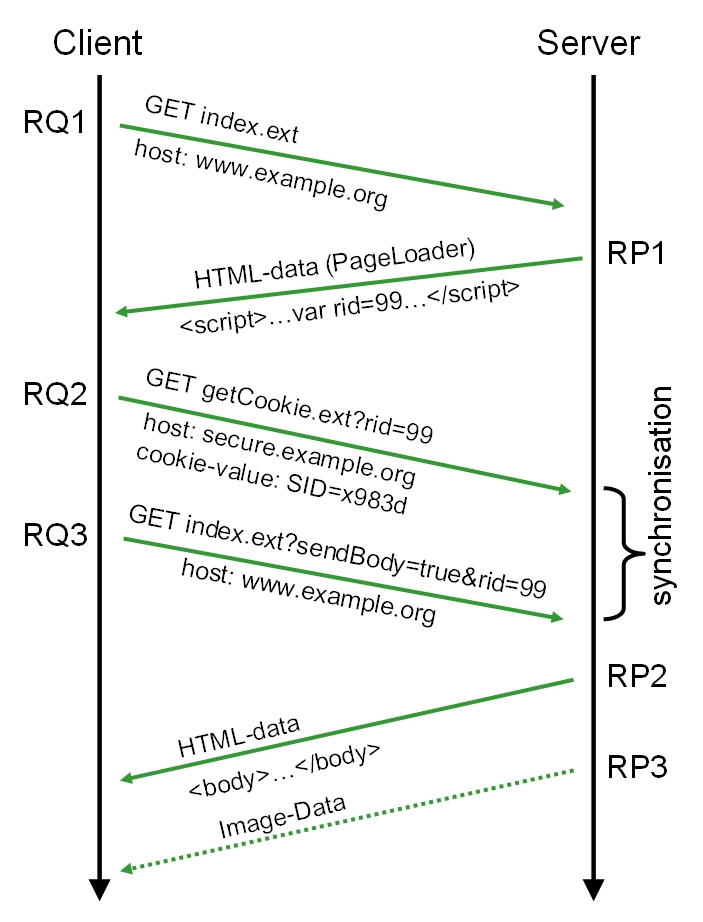
\includegraphics[width=.45\textwidth]{img/sessionsafe-deferred-get2.png}
	}
	\subfloat[Setting the cookie]{
		\label{fig:sessionsafe-deferred-set}
		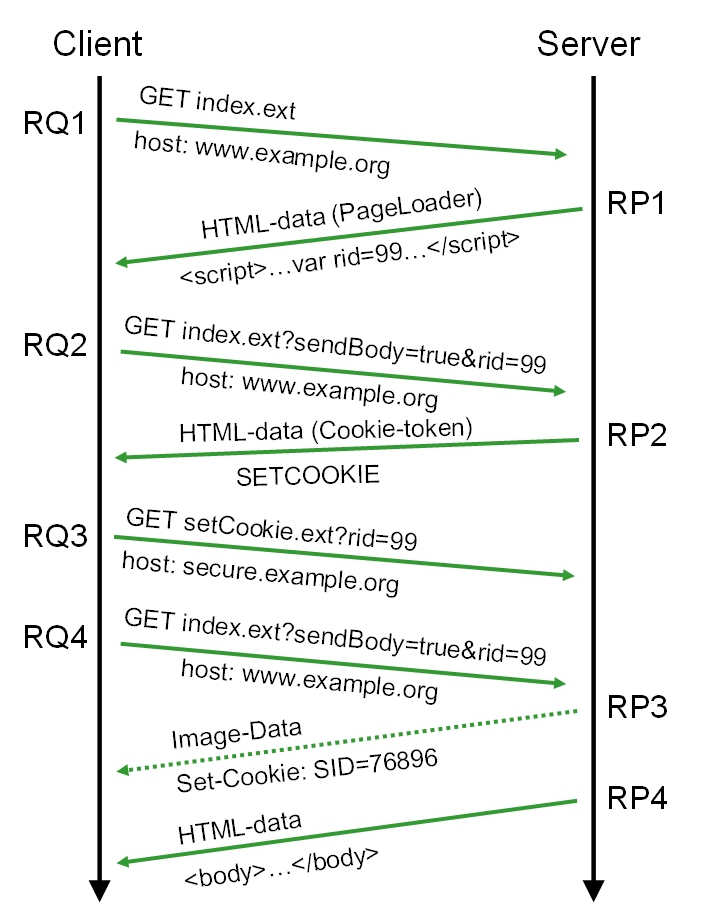
\includegraphics[width=0.45\textwidth]{img/sessionsafe-deferred-set2.png}
	}
	\caption[Deferred loading of a cookie]{Deferred loading of a cookie \cite{Johns2006}}
\end{figure}

Because the cookie needs to be set for a different subdomain than the one the page is served from, it can not simply be included in the \texttt{Set-cookie} header of the HTTP response. Instead, an `image' is included on the returned page, which is served from the domain \url{secure.example.org}. When the user's browser requests the image from this domain, the server is able to set the cookie in the response. The process of setting a cookie is graphically depicted in Figure \ref{fig:sessionsafe-deferred-set}.

Because cookies are set for a different domain than the one web pages are served from, script code which is included in a web page on \url{www.example.com} has no access to cookies stored on the \url{secure.example.com} domain. This prevents attackers from injecting script code (via a \gls{xss} attack) which steals a user's cookie.

Note that this approach does not prevent the attacker from executing a session fixation attack. Indeed, although script code is unable to access cookies stored in a different subdomain, it \emph{is} able to set cookies for its parent domain, as was discussed in section \ref{subdomain-setting}. This allows an attacker to inject script code in a page hosted on \url{www.example.org} that sets a cookie for the domain \url{example.org}. Since \url{secure.example.org} is also a subdomain of \url{example.org}, requests made to this domain will contain the injected cookie.

\subsection{SessionLock}

SessionLock (proposed by Adida et al. in 2008 \cite{Adida2008}) tries to solve session hijacking by making session identifiers only available at the client side. For this purpose, fragment identifiers are used.

Fragment identifiers are included in the URL specification \cite{rfc3986} as a means for making the user's web browser scroll to a certain part of a web page. The fragment identifier is included in the URL as the part that follows the \texttt{\#} character. For example, the URL \url{http://www.example.org/document.html#paragraph4} has \texttt{paragraph4} as its fragment identifier. Loading this URL in the browser will cause the browser to request \emph{document.html} from the web server, and to jump to the element on that page which is identified by the string \texttt{paragraph4}. If no such element is available on the page, the web browser will simply ignore the fragment identifier part of the URL. Fragment identifiers are not sent to the web server on a request, but are available to client-side JavaScript via the \texttt{document.location.hash} \gls{dom} element.

It is in such a fragment identifier that the user's SID will be stored. Interaction between the user's browser and the server happens in the following steps (also depicted in Figure \ref{fig:sessionlock}):
\begin{enumerate}
	\item The user authentication happens over a secure (\gls{https}) connection. When the authentication is successful, the web server sets the SID as a \emph{secure} cookie, and redirects the user to a URL that includes the SID as its fragment identifier.
	\item Subsequent requests are made over an insecure (\gls{http}) connection, and thus do not include the cookie set in the previous step. Instead, the user's browser attaches to every request a \gls{mac}, generated with the (secret) SID, of the tuple \emph{(request-URL, timestamp)}. To avoid having to modify the user's browser to execute these steps, a small piece of JavaScript code is included in the page. This JavaScript code intercepts all user requests, and attaches a timestamp and MAC to every request before it is forwarded to the server.
\end{enumerate}

\begin{figure}[htb]
	\centering
	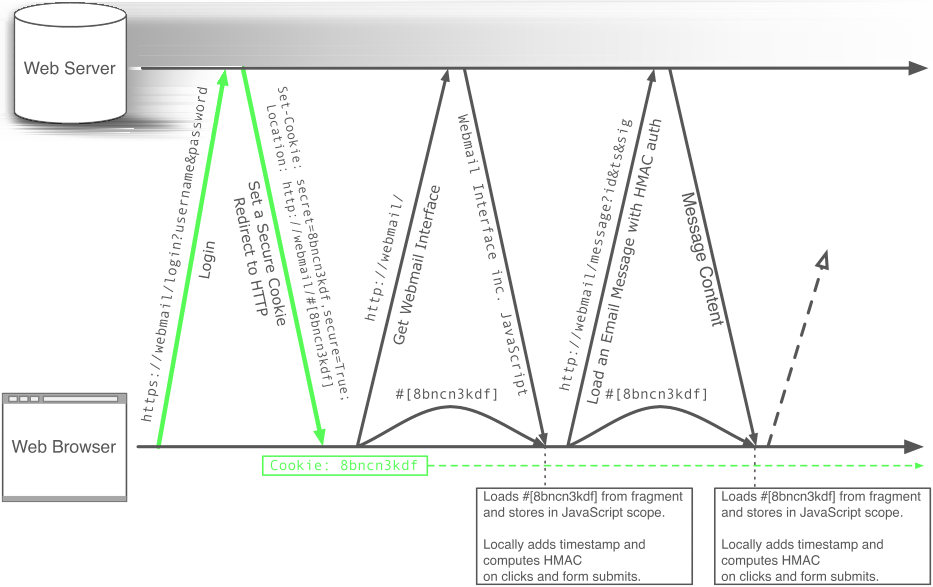
\includegraphics[width=\textwidth]{img/sessionlock.png}
	\caption[The SessionLock protocol]{The SessionLock protocol, with SSL data indicated in green \cite{Adida2008}. Note how the use of the fragment identifier effectively creates a client-only channel from one page to the next.}
	\label{fig:sessionlock}
\end{figure}

By making session identifiers only available at the client side, a \gls{mitm} attacker is not able to capture the SID since it is never sent over the network. The authentication happens over a secure connection because otherwise, the SID would still be sent over an unencrypted channel when it is set by the server. A variant which uses the Diffie-Hellman protocol \cite{Diffie1976} instead of encrypted connections when authenticating is also presented in the paper \cite{Adida2008}.

To make sure that the SID is remembered at the client side, JavaScript code is included in every page returned by the server. This code rewrites all URLs on the page to include the SID as a fragment identifier. Note that the server cannot rewrite these URLs itself, because then the SID would be visible on the network when the page is returned to the client. In case the SID does get lost, JavaScript can still recover it by opening an invisible iframe which loads the URL \url{https://example.org/login/recover} over a secure connection. Within this secure connection, the secure cookie which was set in step 1 will be available. Thus, all the JavaScript code has to do is get the SID value from this cookie, and reload the current page with the SID appended as the fragment identifier.

It is important to note that this session hijacking countermeasure only protects against passive MitM attacks, and against the SID leaking via the \texttt{Referer} header. It does \emph{not} protect the user from accidentally leaking his SID by forwarding a URL \cite{Adida2008}. Moreover, it does \emph{not} protect the user from active attacks. Indeed, since the SID is stored in a way which makes it available to JavaScript, an attacker performing a \gls{xss} attack will still be able to access the SID \cite{Dacosta2011}. For the same reason, the proposed countermeasure does not protect against session fixation either.

Another disadvantage of this approach is that it is only usable for URLs that can be rewritten using JavaScript. Indeed, when binary objects (i.e. Flash) are used to generate dynamic links, URL rewriting will not work \cite{Dacosta2011}.

\subsection{One-time cookies}

In a paper written by Dacosta et al. \cite{Dacosta2011}, a solution to session hijacking is proposed wherein session identifiers are replaced by one-time cookies which are renewed on every request. This is done as follows:
\begin{enumerate}
	\item The user authentication happens over a secure (\gls{https}) connection. In this authentication, a secret seed and a session secret are generated.
	\item Subsequent requests are made over an insecure (\gls{http}) connection. In the $i$-th request, the user's browser attaches the outcome of a hash function  applied $i$ times to the secret seed. Also attached is the current sequence number ($i$, in this case), the user's username, a nonce, and -- most importantly -- a \gls{mac}, generated with the session secret established as part of the authentication, of the triplet \emph{(username, request-URL, hash outcome)}.
\end{enumerate}
It is crucial that the server allows only requests containing a sequence number higher than the last one received. This prevents attackers from replaying captured one-time cookie information. Since the attacker does not know how to generate the next one-time cookie from a previously captured one, and because a previous cookie can not be replayed, the approach renders a captured cookie essentially worthless. Moreover, the request-URL is included in the MAC to make sure that a certain one-time cookie can only be used to access one specific resource.

Aside from preventing session hijacking attacks, this approach will also prevent session fixation attacks. Indeed, as soon as the user authenticates, a new session secret and secret seed -- both unknown to the attacker -- are established. This is similar to renewing the SID on every authentication change.

Because the sequence number is part of the request, the server knows how many times the hash function should be applied to the secret seed. Naturally, the server does not need to apply the hash function $i$ times for every request. Indeed, the computational overhead can be greatly reduced by remembering the previous value, and applying the hash function only $i - i'$ times (where $i'$ is the number of times the function was applied to the previous value) to this previous value.

A major advantage of this approach is that, while users use HTTPS to authenticate (and thus never have their password sent in clear text), a secure connection is not required for subsequent requests. This eliminates the biggest drawback associated with using SSL, namely that of high costs (see section \ref{ssl}).

Possible disadvantages of an approach that uses a new SID for every request were already discussed in section \ref{renewing}. However, two of these do not apply to this particular solution. Firstly, because future SIDs do not need to be explicitly issued by the server, problems with concurrent requests can be avoided by equipping every request with a higher sequence number than the previous one. Secondly, server synchronization is less of a problem because the policy of the servers could be relaxed by allowing any sequence number, as long as it is higher than the last one they received. In this case, subsequent requests by a client could be made to different servers, while synchronization between servers would be limited to the moments a user authenticates. Note that this policy would permit an attacker to replay a one-time cookie, as long as he issues the request to a server different from the one the user issued his request to. Fortunately, the damage is limited by the fact that the one-time cookie can only be used to access one specific resource.

There are also some other disadvantages of one-time cookies. Compared to using regular session IDs over an unencrypted connection, both the client and the server need to perform more computations, and both have to keep more state. However, as is shown in the paper, using secure connections for every request is still much more computationally intensive \cite{Dacosta2011}. Thus, requiring some extra computation compared to using regular session IDs over an unencrypted connection could be considered a minor trade-off to be able to provide secure user authentication.

The paper also describes that in the current implementation, both the server and the client need to be adapted to support one-time cookies. The authors are, however, exploring the idea of modifying one-time cookies to provide a version that does not require a browser extension \cite{Dacosta2011}.

\subsection{Session fixation solution by Johns et al.}

Johns et al. \cite{Johns2011} present a solution to \gls{login session fixation} attacks in the form of a server-side reverse proxy. This allows web applications that have already been deployed in the past to be patched against session fixation afterwards. The proxy works by introducing a second session identifier, called the `proxy session identifier' (or \gls{psid}), which is tightly secured against login session fixation. The proxy works as follows (see Figure \ref{fig:johnsfixation}):
\begin{enumerate}
	\item When a request without a PSID is received by the proxy, it is regarded as the user's first request. In this case, the proxy strips all authentication data from the request and generates a new PSID value. This value is then attached to the server's response via the \texttt{Set-cookie} header.
	\item When a cookie is set by the server (via the \texttt{Set-cookie} header), the proxy associates the PSID that was sent in the request (or the new PSID, if no PSID was present in the request) with the new SID from the server.
	\item When a request containing a SID is received by the proxy, it checks whether the attached PSID is valid for the attached SID. If it is, the PSID is stripped, and the request is forwarded to the web server. If the PSID is not valid, or if no PSID is present, both the PSID and the server's SID are stripped from the request before it is forwarded. This causes the request to be void of any authentication data when it arrives at the server.
	\item To make sure that the PSID is secure against login session fixation attacks, a new PSID is generated -- and sent to the user --- whenever the user changes its authentication state. Note that `changing the authentication state' is not the same as `receiving a new SID from the server', since it is possible that the server does not correctly renew the SID on every authentication state change.
\end{enumerate}

\begin{figure}[htb]
	\centering
	\subfloat[Introducing the PSID]{
		\label{fig:johnsfixation-set}
		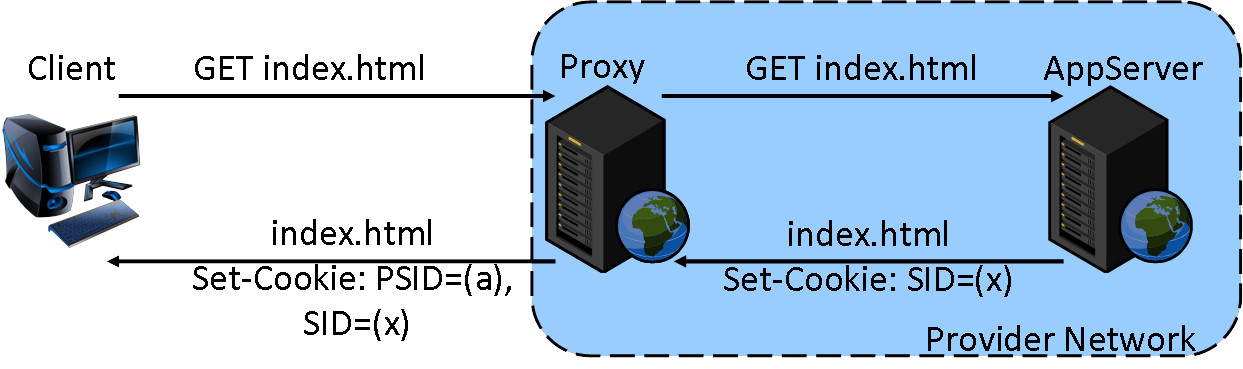
\includegraphics[width=.7\textwidth]{img/johnsfixation-set.png}
	}\\
	\subfloat[Verifying the PSID]{
		\label{fig:johnsfixation-verify}
		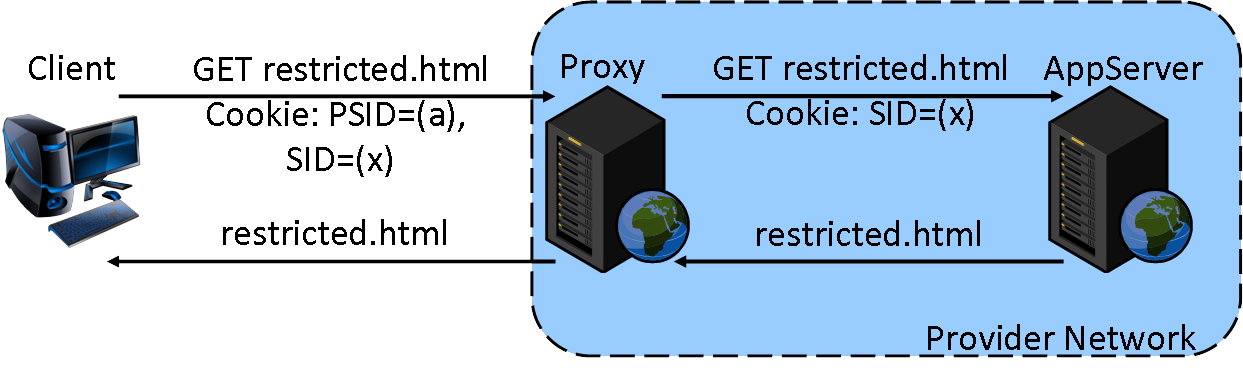
\includegraphics[width=0.7\textwidth]{img/johnsfixation-verify.png}
	}
	\caption[Protecting against login session fixation with a server-side proxy]{\label{fig:johnsfixation}Protecting against login session fixation with a server-side proxy \cite{Johns2011}}
\end{figure}

To see why this solution protects against login session fixation, consider the scenario where the attacker was able to successfully force a SID and PSID upon the victim's browser. As soon as the victim logs in, his PSID is changed by the proxy. When the attacker subsequently tries to make a request using the victim's SID, he is only able to include the old PSID into the request. Because the association between the SID and the old PSID has been invalidated, the proxy will strip the SID from the request before forwarding it to the server. This causes the attacker's request to behave as if it was an unauthenticated request, and prevents the attacker from taking over the victim's session.

To allow the proxy to detect when a user's authentication state changes, the web developer has to configure the proxy with the names of GET and POST parameters that contain password data. When such a parameter is present in a request, the proxy considers it as an authentication request and renews the user's PSID.

The paper mentions that the same solution could also be applied at the framework level, where it is often known which parameters contain password data. The disadvantage of such an approach would be that the solution is then tied to a specific framework, instead of universally deployable. Moreover, if the framework provides session management, a much better solution is to make it renew the SID on every authentication state change itself, instead of introducing a second SID (the PSID).

\section{Client-side countermeasures}

In this section, we focus on session hijacking countermeasures at the client side. The advantage that these approaches have over server-side countermeasures is that they do not require all web application to be secured against this attack. Because of this, it is the \emph{user} who can make sure that he is protected against session hijacking attacks, without having to rely on the web developer of all web applications he uses to implement session hijacking protection. Client-side countermeasures to session \emph{fixation} attacks were, to our knowledge, non-existent at the time of writing \cite{Bonne2011}.

\subsection{SessionShield}\label{sessionshield} %TODO

SessionShield is a client-side proxy providing protection against session hijacking attacks. It was proposed by Nikiforakis et al. in 2010 \cite{Nikiforakis2010}. SessionShield is based on the idea that session identifiers should not be available to script code running in a user's browser.

The proxy keeps session cookies unavailable to script code by separating them from the browser. It does this as follows (see Figure \ref{fig:nikiforakis}):
\begin{enumerate}
	\item When a session cookie is set by the server (via the \texttt{Set-cookie} header), the proxy stores this cookie in his internal database, and strips it from the response before it is sent to the client.
	\item On every outgoing request, the proxy queries its internal database using the domain of the request as the key and adds to the outgoing request all cookies for this domain that are present in the database.
\end{enumerate}

\begin{figure}[htb]
	\centering
	\subfloat[An incoming response containing a new SID.]{
		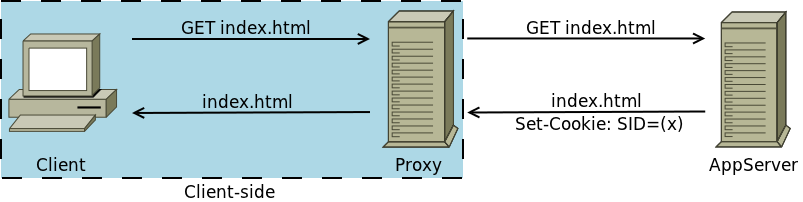
\includegraphics[width=.7\textwidth]{img/nikiforakis-set.png}
		\label{fig:clientside-request}
	}\\
	\subfloat[An outgoing request by the browser does not contain any cookies. The proxy attaches the cookies for this domain that were stored in the database.]{
		\label{fig:clientside-response}
		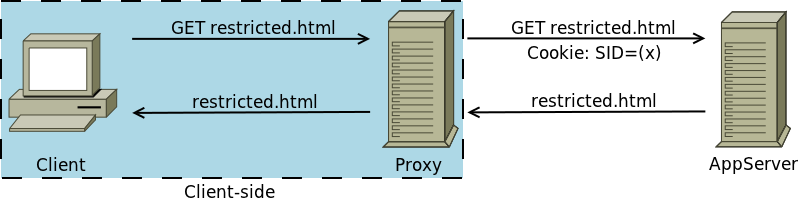
\includegraphics[width=0.7\textwidth]{img/nikiforakis-get.png}
	}
	\caption{Protecting against session hijacking with a client-side proxy}
	\label{fig:nikiforakis}
\end{figure}

To identify which cookies are session cookies, SessionShield uses a sophisticated SID detection algorithm. This algorithm considers a cookie to be a session cookie in one of the following cases:
\begin{itemize}
	\item The name of the cookie is in a list of known session identifiers, such as \texttt{phpsessid}, \texttt{aspsessionid} and \texttt{jspsession}.
	\item The name of the cookie contains the substring ``sess'', and the value is more than 10 characters long.
	\item The value of the cookie passes a `SID probability check', which consists of checking the string's information entropy, its correlation with the uniform distribution, and the number of dictionary words contained in it.
\end{itemize}

SessionShield works in much the same way as \texttt{HttpOnly} cookies, but takes it one step further: it makes sure that cookies will never be visible in the browser, preventing an attacker from reading cookies even if he is able to seize control over the victim's browser in any way. This not only prevents session hijacking via \gls{xss} attacks, it also prevents rogue browser extensions from capturing a user's session cookie \cite{TerLouw2007}. Another advantage SessionShield has over HttpOnly is that it works at the client side, allowing the user to be secure even when the web application fails to set the \texttt{HttpOnly} flag for all session cookies.

A disadvantage of implementing SessionShield as a proxy occurs when different browsers are using SessionShield at the same time. In this case, the proxy will attach cookies that were set for one browser to the other browser's outgoing requests, causing the user to be authenticated in both browsers when he has only explicitly logged in with one of them. Moreover, clearing private data in the browser, or using the browser's `private browsing' functionality, has no effect on SessionShield, causing the user to be authenticated even when he expects not to be. We will discuss other advantages and disadvantages of implementing such a policy as a browser extension instead of a proxy in the next chapter.

\subsection{Noxes}\label{noxes}

Noxes, developed by by Kirda et al. in 2006, is a client-side solution to mitigate cross-site scripting attacks \cite{Kirda2006}, and should technically be described in the next section. However, since it is developed specifically to prevent information leakage from one domain to another, we discuss it here.

Noxes works similar to a personal firewall like ZoneAlarm\footnote{ZoneAlarm is available from \url{http://www.zonealarm.com/}.} or Windows Firewall\footnote{Windows Firewall is included by default on every version of Microsoft Windows since Windows XP Service Pack 2. More information is available on \url{http://technet.microsoft.com/en-us/network/bb545423.aspx}.}. However, instead of controlling the connections for all processes running on a user's machine, it only handles requests made by the user's browser. This allows Noxes to offer more fine-grained controls which are specifically tailored to web applications. For example, whenever a JavaScript request is trying to send information to a domain that is not known by Noxes, the user is presented with a prompt that asks for user confirmation. The user is able to accept or deny the request, and to create a firewall rule for similar future requests.

This approach is obviously very cumbersome: the user will have to explicitly allow every request that is made to a different domain. Because of this, Noxes includes a list of safe scenarios. When such a scenario occurs, the request is allowed without consulting the user. The following scenarios are considered safe:
\begin{description}
	\item[Requests to the same domain] When the base domains of the request and the page the request originated from are the same, information leakage to another domain is not possible. Noxes checks whether a request originated from the same domain by comparing the \texttt{Referer} HTTP header of the request to the domain of the requested web page.
	\item[Static links] When links do not contain dynamic components, an attacker is unable to embed the victim's SID as part of the URL. Indeed, an attacker can only create the URL after he has read the domain's cookie value, which then has to be dynamically included in the URL.
\end{description}
Static links do not completely prevent a SID from leaking to another domain. Because of this, Noxes includes two exceptions to the second `safe rule'. Firstly, consider the scenario where an attacker includes in the web page a static link to his own domain for each of the two possible bit values for every bit in the SID. He is then able to use JavaScript to load the links that correspond to the individual bits in the SID, one by one (see Figure \ref{Noxes-attack}). Because of this, Noxes allows maximally $k$ static links to the same external domain, where $k$ is a customizable threshold.

\begin{figure}
\begin{lstlisting}[language=HTML]
<html>
...
<img src="http://attacker.com/bit0_0.jpg">
<img src="http://attacker.com/bit0_1.jpg">
<img src="http://attacker.com/bit1_0.jpg">
<img src="http://attacker.com/bit1_1.jpg">
...
<script>
    for [i=0 to 100] {
        if (cookiebits[i] == 0)
            <contact http://attacker.com/biti_0.jpg>
        else if (cookiebits[i] == 1)
            <contact http://attacker.com/biti_1.jpg>
    }
</script>
</html>
\end{lstlisting}
	\caption[Using static links to transmit the SID to an attacker's domain]{\label{Noxes-attack}Pseudo code for a JavaScript-based attack that transmits the SID to an attacker's domain using only static links (based on \cite{Kirda2006})}
\end{figure}

A second exception to the second `safe rule' is made for pop-up and pop-under windows to a different domain. Using these, an attacker can open a window containing a static link to a page on his own domain, only to afterwards set the window's title to the value of the victim's cookie. This makes him able to read the cookie value from within his own page, by using JavaScript on his own page to access the value of the \texttt{document.title} attribute. Because of this, Noxes presents an alert message to the user when it detects that a pop-up or pop-under window to a different domain is opened, regardless of the link being static.

Unfortunately, Noxes' complete policy still allows an attacker to leak the victim's SID to his own domain. Indeed, as Nikiforakis already noted \cite{Nikiforakis2010}, an attacker can create a XSS attack which, instead of \texttt{<script>} tags, injects an HTML-tag which statically references a URL to the attackers domain including the SID value. Furthermore, an attacker is able to make the victim's browser load multiple pages of the originating domain, with every page sending maximally $k$ characters ($k$ being the maximum of allowed outgoing links to an external domain) of the victim's SID to the attacker's server.

Another problem with Noxes is that it uses the \texttt{Referer} header to check whether a request comes from a different domain than the one of the requested web page. As we saw in section \ref{leaking-via-referer}, the \texttt{Referer} header is often stripped \cite{Barth2008}. This will cause Noxes to present an alert even for some requests that go to the same domain as the one they originated from.

It can be concluded that Noxes is too complex to be considered a long-time solution against session hijacking attacks. Firstly, user interaction is needed for many requests, which is often cumbersome for the user. Moreover, less technically inclined users will not be able to judge whether a request is safe or not. Secondly, as can be seen from the `safe rule' exceptions, lots of possible attack vectors will have to be accounted for by the firewall. This will cause Noxes to be often lacking in security.

\subsection{Dynamic tainting and static analysis}

Similar to Noxes, the solution developed by Vogt et al. \cite{Vogt2007} that we will describe here is actually meant to mitigate data leakage in XSS attacks. It uses a combination of dynamic data tainting and static analysis to prevent sensitive data (e.g. session cookies) from leaking to a different domain than the one it originated from.

Tainting is a technique which makes sure that sensitive data keeps being regarded as such, even when it is passed around. For this, sensitive data is given a `taint', which is propagated when (part of) the tainted data is assigned to a different variable, or used as part in an arithmetic or logic operation. For example, consider the following snippet of JavaScript code, wherein \texttt{document.cookie} is tainted:
\begin{lstlisting}[language=JavaScript]
var arr = []; // arr.length = 0
if (document.cookie[0] == 'a')
    arr[0] = 1;
if (arr.length == 1)
    y = 'a';
\end{lstlisting}
Because \texttt{document.cookie} is tainted, \texttt{arr} will be tainted as soon as the first if-test is executed. Upon executing the second if-test, \texttt{y} is also tainted, which correctly indicates that information about the sensitive (cookie) data is present in this variable.

When it is detected that a web page tries to send tainted data to a third party, the user is asked to allow or deny the actual transmission of this data, much in the same way as was the case with Noxes. Sending of tainted data to a third party can be achieved in many ways. Some examples of the methods the countermeasure detects are changing the location of the current web page, changing the source of an image, and automatically submitting a form \cite{Vogt2007}.

Unfortunately, several hidden channels that can be used to transmit sensitive information remain undetected by this solution \cite{Nikiforakis2010}. Moreover, Russo et al. described how the protection technique can be circumvented by both encoding secret information into the structure of the \gls{dom} tree and exploiting tree navigation \cite{Russo2009}. Another disadvantage of this solution stems from the fact that it needs to ask for user confirmation. This leads to the problems which were already discussed when describing Noxes.

% TODO: conclusie en comparison-tabel. Zeg ook iets dat session fixation bijina nooit solved is, en dat voor de oplossingen waarvoor eht wel zo is server moet aangepast worden.

\begin{table}[htbp]
	\centering
	\begin{tabularx}{\textwidth}{r|cccc}
		& Needs & Prevents & Prevents\\
		& modification & session hijacking & session fixation\\
		\hline
		Deferred loading & server & via JavaScript & no\\
		SessionLock & server & via MitM \& \texttt{Referer} & no\\
		One-time cookies & server \& client & yes\footnote{When using the same server for every request, session hijacking is prevented entirely. When using different servers, an attacker is prevented from accessing a resource different from the one the victim used the SID for.} & yes\\
		Johns et al. & server & no & yes\\
		SessionShield & client & &\\
		Noxes & & &\\
		Dynamic tainting & & &\\
	\end{tabular}
	\caption{Comparison of different session attack countermeasures}
	\label{tab:countermeasures}
\end{table}

\section{Script injection countermeasures}\label{xss-countermeasures}

Over the years, different solutions to \gls{xss} have been proposed, both at the server and at the client side. In this section, we describe the general principles behind these approaches, without going into too much details.

\subsection{Server-side countermeasures}

At the server side, two general categories of XSS countermeasures exist. The first one is that of \emph{input validation}, or \emph{input filtering}, as is available in solutions like Sanctum's AppShield \cite{Klein2002}. In such an approach, all script code is stripped from user input, in order to prevent any user-submitted executable code to be sent to the browser. This is done either by removing certain substrings (e.g. \texttt{<script>} tags), or by replacing characters with their HTML-safe counterparts (e.g. replacing \texttt{<} by \texttt{\&lt;} and \texttt{>} by \texttt{\&gt;}), which will be converted back to the original character once they are rendered by the browser.

A second category of server-side XSS countermeasures tries to detect user-injected script code when it is returned to the victim. One solution that does this is XSS-Guard, developed by Bisht et al. \cite{Bisht2008}. In this solution, two versions are generated for every returned page: one without, and one containing user input. XSS-Guard then compares both pages to see if there are any differences in JavaScript between the two pages. If differences are found, the relevant parts are stripped from the response before it is sent to the client. This prevents JavaScript in the user-input from being returned to the client.

Another such solution, called SWAP, was presented by Wurzinger et al. in 2009 \cite{Wurzinger2009}. It works by assigning a so-called `script ID' to every piece of JavaScript generated by the server. When script code is found in a server response, it is checked whether it has a valid script ID associated to it. If it does, the response is forwarded to the client. If the piece of code does not correspond to a valid script ID, the response is discarded, and the user is presented with a screen that notifies him of the suspected XSS attack.

For both categories of server-side countermeasures, a mechanism that automatically detects JavaScript is needed: the first category needs it to find JavaScript in user input, whereas the second category needs it to detect JavaScript in a returned page. A difficulty in detecting JavaScript is that it has to be able to recognize all different ways in which script code can be injected (see section \ref{injecting-script} and \cite{Jim2007}), including all possible encodings and taking into account differences in various browsers (called \emph{browser quirks}). AppShield approaches this difficulty by using pattern matching on known attack vectors \cite{Klein2002}, whereas both XSS-Guard and SWAP use Firefox's HTML parser to detect which parts of a web page contain script code that will be executed by Firefox \cite{Bisht2008,Wurzinger2009}. While the first approach will possibly overlook some attack vectors, the second approach will cause every piece of HTML that will trigger code to be executed in the Firefox web browser to be detected. A disadvantage of the second approach, however, is that it does not take into account differences between various browsers. This makes it possible that, even if Firefox does not consider a particular piece of HTML code to be valid JavaScript, another browser might execute it as script code. Hence, an attacker will still be able to bypass the proxy by injecting JavaScript code which is specific to the Internet Explorer web browser.

A disadvantage shared by both approaches in the second category is that they do not prevent binary Flash objects from being injected. Thus, an attacker will still be able to use Flash to inject JavaScript on a page, regardless of the countermeasure being in use \cite{Bisht2008,FlashJSattack}.

Another disadvantage, limited to SWAP, is that an attacker will still be able to inject script code in order to execute a \gls{dos} attack. Indeed, because script code is only detected \emph{after} it has been injected at the server, an attacker is still able to inject script code. Moreover, because server responses containing injected code are discarded entirely by SWAP, all responses containing the attacker's injected code will be prevented from being sent to the client. As such, injecting script code now allows an attacker to render a page unavailable to the users of a website.

\subsection{Client-side countermeasures}

At the client side, four important countermeasures have been developed to mitigate cross-site scripting. Two of them, Noxes and dynamic tainting, were already discussed in the previous section. We discuss the remaining two countermeasures here.

The simplest countermeasure, called NoScript, allows the user to choose for each piece of script code whether it should be allowed to be executed \cite{NoScript}. It also provides specific protection to XSS attacks. Furthermore, allows other plugins and embeddings (e.g. Java and Flash) to be blocked. By default, it uses a whitelist approach, which implies that all scripts are blocked by default unless the user manually specifies an exception for a particular piece of JavaScript. As was already described in the context of Noxes, this is very cumbersome, especially for less technically inclined users. Moreover, it has been shown that a XSS vulnerability on a NoScript domain can be used to run JavaScript from any website, despite NoScript being enabled \cite{NoScriptCriticism}.

A second countermeasure, called HProxy and developed by Nikiforakis et al. \cite{Nikiforakis2010a} was originally developed to prevent SSL stripping attacks. In such an attack, the attacker acts as an active \gls{mitm} to force users to communicate over an insecure channel with the web server. To detect such attacks, HProxy compares different HTML and HTTP elements in the response from the server that could be misused by a MitM attacker to what they looked like in previous page responses. What is relevant for our discussion is that one of these elements is JavaScript code, which is checked as follows:
\begin{enumerate}
	\item When the first response is received by the server, a second request is made by HProxy. The first response is then compared to the second one in order to identify the dynamic JavaScript parts of the web page, i.e. the parts of the script code that differ on every page request.
	\item For all subsequent responses, it is checked whether any non-dynamic JavaScript on the page differs from the JavaScript returned in the first response. If it does, the web page is marked as `unsafe', and the response is dropped.
\end{enumerate}
While HProxy is definitely a step in the right direction, enabling users to be secure against XSS attacks without requiring support from the web application, it does have some disadvantages. Firstly, current versions of web pages are always compared to the first version that was received. This causes updated versions of websites to be blocked. Moreover, it prevents the detection of attacks that occur the first time a page is loaded when HProxy is in use. A second disadvantage is that HProxy suffers from false positives: the paper mentions that, even with advanced JavaScript change detection\footnote{The advanced JavaScript change detection consists of the practices described in this section, together with the whitelisting of signed scripts, as is described in the next section. Without the whitelisting in place, false positives occurred for about 8\% of legitimate responses} in place, 3\% of legitimate server responses are mistaken for malicious responses.

\subsection{Hybrid approaches}

Hybrid approaches mitigate XSS attacks by letting the server define a policy, while making the client check whether a returned page adheres to this policy.

`Signed scripts', proposed by Mozilla \cite{SignedScripts}, provide a way for web servers to digitally sign the scripts they send to a client. The client is then able to verify that the scripts which are present in a web page are actually issued by the web server, and not modified in transit by an attacker. Currently, signed scripts are used by the Firefox web browser to allow a script to request extended privileges (e.g. modifying the browser's preferences). However, signed scripts are also used by HProxy, described earlier, to reduce the number of false positives by always allowing a correctly signed script to be executed.

Another hybrid approach is that of `Browser Enforced Embedded Policies' (or BEEP for short), developed by Jim et al. in 2007 \cite{Jim2007}. Here, the server includes an additional JavaScript function in the response, which will enable the browser to check that the page it is included in does not include injected code. Whenever a browser that enforces BEEP encounters a script while rendering a page, it invokes this special function with an identifier of the JavaScript code as its argument. If the function returns \texttt{true} then the script is deemed acceptable and will be executed; otherwise it will be ignored. The browser describes two possible policies that can be implemented in such a JavaScript function: \emph{whitelisting}, in which the function returns \texttt{true} if the SHA1 hash of its argument corresponds with one of the `safe hashes' included in a whitelist, and \emph{\gls{dom} sandboxing}, in which parts of the web page that include user content are marked by setting their \texttt{class} attribute to \texttt{noexecute}. In this second policy, the function checks that its argument is not part of such a sandbox, and returns \texttt{false} if it is, preventing execution of the JavaScript code.

